\documentclass{whiteboard}
\begin{document}
\begin{frame}[plain,t]
\bbcover{Grafos}{Árvore Geradora Mínima: Definição}{Prof. Edson Alves}{Faculdade UnB Gama}

\end{frame}
\begin{frame}[plain,t]
\begin{tikzpicture}
\node[draw,opacity=0] at (0, 0) {x};
\node[draw,opacity=0] at (14, 8) {x};

	\node[anchor=west] (title) at (0.0, 6.0) { \Large \bbbold{Árvores geradoras} };
\end{tikzpicture}
\end{frame}
\begin{frame}[plain,t]
\begin{tikzpicture}
\node[draw,opacity=0] at (0, 0) {x};
\node[draw,opacity=0] at (14, 8) {x};

	\node[anchor=west] (title) at (0.0, 6.0) { \Large \bbbold{Árvores geradoras} };

	\node[anchor=west] (a) at (1.0, 5.0) { \bbtext{Seja $G(V, E)$ um grafo. Uma \bbbold{árvore geradora} de $G$ é um subgrafo $T(V, E')$} };

	\node[anchor=west] (b) at (0.5, 4.25) { \bbtext{de $G$ tal que $T$ é uma árvore que contém todos os vértices de $G$.} };

\end{tikzpicture}
\end{frame}
\begin{frame}[plain,t]
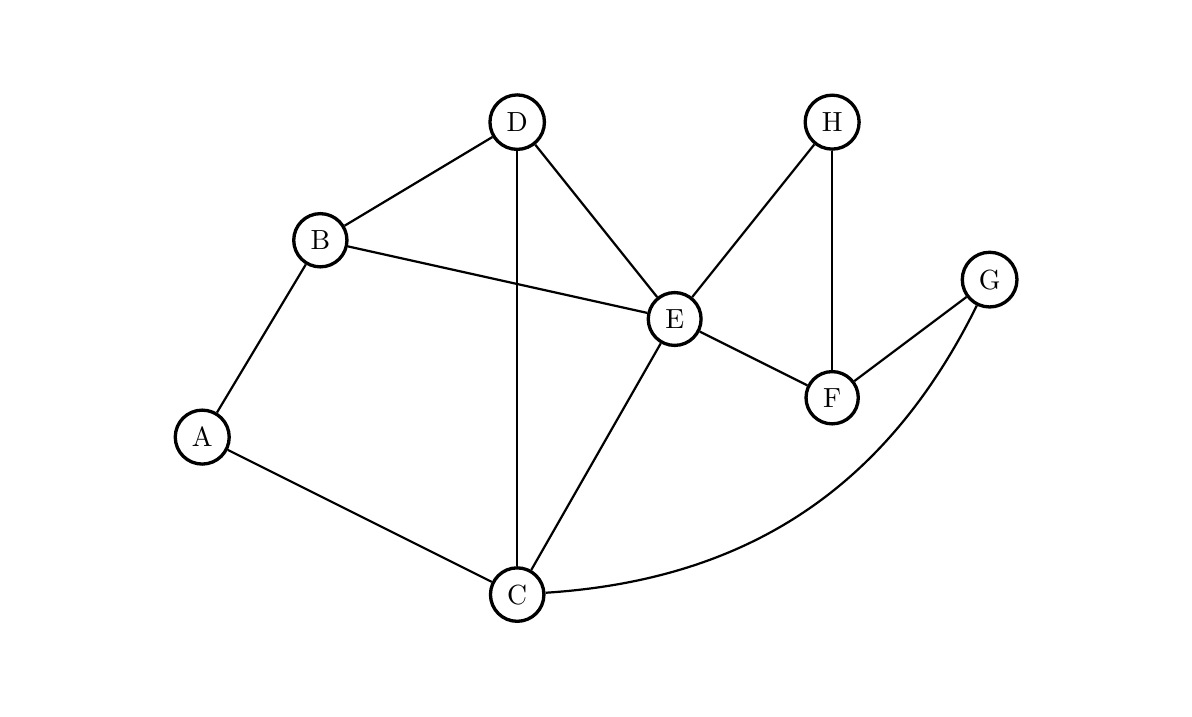
\begin{tikzpicture}
\node[draw,opacity=0] at (0, 0) {x};
\node[draw,opacity=0] at (14, 8) {x};

	\node[draw,very thick,circle] (nodeA) at (2.0, 3.0) { \bbtext{A} };

	\node[draw,very thick,circle] (nodeB) at (3.5, 5.5) { \bbtext{B} };

	\node[draw,very thick,circle] (nodeC) at (6.0, 1.0) { \bbtext{C} };

	\node[draw,very thick,circle] (nodeD) at (6.0, 7.0) { \bbtext{D} };

	\node[draw,very thick,circle] (nodeE) at (8.0, 4.5) { \bbtext{E} };

	\node[draw,very thick,circle] (nodeF) at (10.0, 3.5) { \bbtext{F} };

	\node[draw,very thick,circle] (nodeG) at (12.0, 5.0) { \bbtext{G} };

	\node[draw,very thick,circle] (nodeH) at (10.0, 7.0) { \bbtext{H} };

	\draw[thick](nodeA) to (nodeB);

	\draw[thick](nodeA) to (nodeC);

	\draw[thick](nodeB) to (nodeD);

	\draw[thick](nodeB) to (nodeE);

	\draw[thick](nodeC) to (nodeD);

	\draw[thick](nodeC) to (nodeE);

	\draw[thick](nodeC) to [bend right] (nodeG);

	\draw[thick](nodeD) to (nodeE);

	\draw[thick](nodeE) to (nodeF);

	\draw[thick](nodeE) to (nodeH);

	\draw[thick](nodeF) to (nodeG);

	\draw[thick](nodeF) to (nodeH);

\end{tikzpicture}
\end{frame}
\begin{frame}[plain,t]
\begin{tikzpicture}
\node[draw,opacity=0] at (0, 0) {x};
\node[draw,opacity=0] at (14, 8) {x};

	\node[draw,very thick,circle] (nodeA) at (2.0, 3.0) { \bbtext{A} };

	\node[draw,very thick,circle] (nodeB) at (3.5, 5.5) { \bbtext{B} };

	\node[draw,very thick,circle] (nodeC) at (6.0, 1.0) { \bbtext{C} };

	\node[draw,very thick,circle] (nodeD) at (6.0, 7.0) { \bbtext{D} };

	\node[draw,very thick,circle] (nodeE) at (8.0, 4.5) { \bbtext{E} };

	\node[draw,very thick,circle] (nodeF) at (10.0, 3.5) { \bbtext{F} };

	\node[draw,very thick,circle] (nodeG) at (12.0, 5.0) { \bbtext{G} };

	\node[draw,very thick,circle] (nodeH) at (10.0, 7.0) { \bbtext{H} };

	\draw[thick](nodeA) to (nodeB);

	\draw[thick,very thick,dashed,color=BBCyan](nodeA) to (nodeC);

	\draw[thick](nodeB) to (nodeD);

	\draw[thick,very thick,dashed,color=BBCyan](nodeB) to (nodeE);

	\draw[thick,very thick,dashed,color=BBCyan](nodeC) to (nodeD);

	\draw[thick,very thick,dashed,color=BBCyan](nodeC) to (nodeE);

	\draw[thick](nodeC) to [bend right] (nodeG);

	\draw[thick](nodeD) to (nodeE);

	\draw[thick,very thick,dashed,color=BBCyan](nodeE) to (nodeF);

	\draw[thick](nodeE) to (nodeH);

	\draw[thick,very thick,dashed,color=BBCyan](nodeF) to (nodeG);

	\draw[thick,very thick,dashed,color=BBCyan](nodeF) to (nodeH);





\end{tikzpicture}
\end{frame}
\begin{frame}[plain,t]
\begin{tikzpicture}
\node[draw,opacity=0] at (0, 0) {x};
\node[draw,opacity=0] at (14, 8) {x};

	\node[anchor=west] (title) at (0.0, 6.0) { \Large \bbbold{Árvore mínima geradora} };
\end{tikzpicture}
\end{frame}
\begin{frame}[plain,t]
\begin{tikzpicture}
\node[draw,opacity=0] at (0, 0) {x};
\node[draw,opacity=0] at (14, 8) {x};

	\node[anchor=west] (title) at (0.0, 6.0) { \Large \bbbold{Árvore mínima geradora} };

	\node[anchor=west] (a) at (1.0, 5.0) { \bbtext{Seja $G(V, E)$ um grafo ponderado. Uma árvore geradora $T(V, E')$ de $G$ é} };

	\node[anchor=west] (b) at (0.5, 4.25) { \bbtext{uma \bbbold{árvore mínima geradora} (MST) de $G$ se a soma} };

	\node[] (c) at (7.0, 3.25) { $\displaystyle c(T) = \sum_{e\in E'} w(e)$ };

	\node[anchor=west] (d) at (0.5, 2.5) { \bbtext{é mínima.} };

\end{tikzpicture}
\end{frame}
\begin{frame}[plain,t]
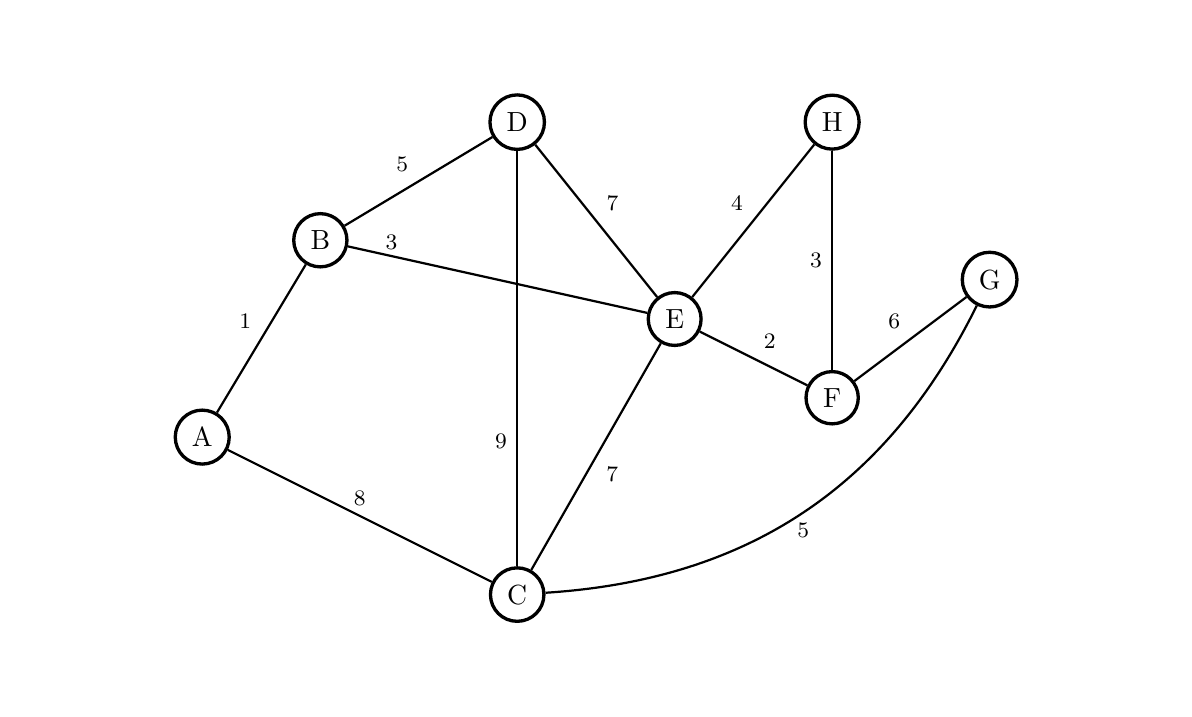
\begin{tikzpicture}
\node[draw,opacity=0] at (0, 0) {x};
\node[draw,opacity=0] at (14, 8) {x};

	\node[draw,very thick,circle] (nodeA) at (2.0, 3.0) { \bbtext{A} };

	\node[draw,very thick,circle] (nodeB) at (3.5, 5.5) { \bbtext{B} };

	\node[draw,very thick,circle] (nodeC) at (6.0, 1.0) { \bbtext{C} };

	\node[draw,very thick,circle] (nodeD) at (6.0, 7.0) { \bbtext{D} };

	\node[draw,very thick,circle] (nodeE) at (8.0, 4.5) { \bbtext{E} };

	\node[draw,very thick,circle] (nodeF) at (10.0, 3.5) { \bbtext{F} };

	\node[draw,very thick,circle] (nodeG) at (12.0, 5.0) { \bbtext{G} };

	\node[draw,very thick,circle] (nodeH) at (10.0, 7.0) { \bbtext{H} };

	\draw[thick](nodeA) to node[above left] { \footnotesize \bbinfo{1} } (nodeB);

	\draw[thick](nodeA) to node[above] { \footnotesize \bbinfo{8} } (nodeC);

	\draw[thick](nodeB) to node[above left] { \footnotesize \bbinfo{5} } (nodeD);

	\draw[thick](nodeB) to node[above left,pos=0.2] { \footnotesize \bbinfo{3} } (nodeE);

	\draw[thick](nodeC) to node[left,pos=0.3] { \footnotesize \bbinfo{9} } (nodeD);

	\draw[thick](nodeC) to node[below right] { \footnotesize \bbinfo{7} } (nodeE);

	\draw[thick](nodeC) to [bend right] node[below] { \footnotesize \bbinfo{5} } (nodeG);

	\draw[thick](nodeD) to node[above right] { \footnotesize \bbinfo{7} } (nodeE);

	\draw[thick](nodeE) to node[above right] { \footnotesize \bbinfo{2} } (nodeF);

	\draw[thick](nodeE) to node[above left] { \footnotesize \bbinfo{4} } (nodeH);

	\draw[thick](nodeF) to node[above left] { \footnotesize \bbinfo{6} } (nodeG);

	\draw[thick](nodeF) to node[left] { \footnotesize \bbinfo{3} } (nodeH);

\end{tikzpicture}
\end{frame}
\begin{frame}[plain,t]
\begin{tikzpicture}
\node[draw,opacity=0] at (0, 0) {x};
\node[draw,opacity=0] at (14, 8) {x};

	\node[draw,very thick,circle] (nodeA) at (2.0, 3.0) { \bbtext{A} };

	\node[draw,very thick,circle] (nodeB) at (3.5, 5.5) { \bbtext{B} };

	\node[draw,very thick,circle] (nodeC) at (6.0, 1.0) { \bbtext{C} };

	\node[draw,very thick,circle] (nodeD) at (6.0, 7.0) { \bbtext{D} };

	\node[draw,very thick,circle] (nodeE) at (8.0, 4.5) { \bbtext{E} };

	\node[draw,very thick,circle] (nodeF) at (10.0, 3.5) { \bbtext{F} };

	\node[draw,very thick,circle] (nodeG) at (12.0, 5.0) { \bbtext{G} };

	\node[draw,very thick,circle] (nodeH) at (10.0, 7.0) { \bbtext{H} };

	\draw[thick,very thick,dashed,color=BBCyan](nodeA) to node[above left] { \footnotesize \bbinfo{1} } (nodeB);

	\draw[thick](nodeA) to node[above] { \footnotesize \bbinfo{8} } (nodeC);

	\draw[thick,very thick,dashed,color=BBCyan](nodeB) to node[above left] { \footnotesize \bbinfo{5} } (nodeD);

	\draw[thick,very thick,dashed,color=BBCyan](nodeB) to node[above left,pos=0.2] { \footnotesize \bbinfo{3} } (nodeE);

	\draw[thick](nodeC) to node[left,pos=0.3] { \footnotesize \bbinfo{9} } (nodeD);

	\draw[thick,very thick,dashed,color=BBCyan](nodeC) to node[below right] { \footnotesize \bbinfo{7} } (nodeE);

	\draw[thick,very thick,dashed,color=BBCyan](nodeC) to [bend right] node[below] { \footnotesize \bbinfo{5} } (nodeG);

	\draw[thick](nodeD) to node[above right] { \footnotesize \bbinfo{7} } (nodeE);

	\draw[thick,very thick,dashed,color=BBCyan](nodeE) to node[above right] { \footnotesize \bbinfo{2} } (nodeF);

	\draw[thick](nodeE) to node[above left] { \footnotesize \bbinfo{4} } (nodeH);

	\draw[thick](nodeF) to node[above left] { \footnotesize \bbinfo{6} } (nodeG);

	\draw[thick,very thick,dashed,color=BBCyan](nodeF) to node[left] { \footnotesize \bbinfo{3} } (nodeH);









\end{tikzpicture}
\end{frame}
\begin{frame}[plain,t]
\begin{tikzpicture}
\node[draw,opacity=0] at (0, 0) {x};
\node[draw,opacity=0] at (14, 8) {x};

	\node[draw,very thick,circle] (nodeA) at (2.0, 3.0) { \bbtext{A} };

	\node[draw,very thick,circle] (nodeB) at (3.5, 5.5) { \bbtext{B} };

	\node[draw,very thick,circle] (nodeC) at (6.0, 1.0) { \bbtext{C} };

	\node[draw,very thick,circle] (nodeD) at (6.0, 7.0) { \bbtext{D} };

	\node[draw,very thick,circle] (nodeE) at (8.0, 4.5) { \bbtext{E} };

	\node[draw,very thick,circle] (nodeF) at (10.0, 3.5) { \bbtext{F} };

	\node[draw,very thick,circle] (nodeG) at (12.0, 5.0) { \bbtext{G} };

	\node[draw,very thick,circle] (nodeH) at (10.0, 7.0) { \bbtext{H} };

	\draw[thick,very thick,dashed,color=BBCyan](nodeA) to node[above left] { \footnotesize \bbinfo{1} } (nodeB);

	\draw[thick](nodeA) to node[above] { \footnotesize \bbinfo{8} } (nodeC);

	\draw[thick,very thick,dashed,color=BBCyan](nodeB) to node[above left] { \footnotesize \bbinfo{5} } (nodeD);

	\draw[thick,very thick,dashed,color=BBCyan](nodeB) to node[above left,pos=0.2] { \footnotesize \bbinfo{3} } (nodeE);

	\draw[thick](nodeC) to node[left,pos=0.3] { \footnotesize \bbinfo{9} } (nodeD);

	\draw[thick,very thick,dashed,color=BBCyan](nodeC) to node[below right] { \footnotesize \bbinfo{7} } (nodeE);

	\draw[thick,very thick,dashed,color=BBCyan](nodeC) to [bend right] node[below] { \footnotesize \bbinfo{5} } (nodeG);

	\draw[thick](nodeD) to node[above right] { \footnotesize \bbinfo{7} } (nodeE);

	\draw[thick,very thick,dashed,color=BBCyan](nodeE) to node[above right] { \footnotesize \bbinfo{2} } (nodeF);

	\draw[thick](nodeE) to node[above left] { \footnotesize \bbinfo{4} } (nodeH);

	\draw[thick](nodeF) to node[above left] { \footnotesize \bbinfo{6} } (nodeG);

	\draw[thick,very thick,dashed,color=BBCyan](nodeF) to node[left] { \footnotesize \bbinfo{3} } (nodeH);










	\node[] (info) at (1.0, 7.0) { $\displaystyle c(T) = 32$ };

\end{tikzpicture}
\end{frame}
\begin{frame}[plain,t]
\begin{tikzpicture}
\node[draw,opacity=0] at (0, 0) {x};
\node[draw,opacity=0] at (14, 8) {x};

	\node[anchor=west] (title) at (0.0, 7.0) { \Large \bbbold{Propriedades da árvore mínima geradora} };

\end{tikzpicture}
\end{frame}
\begin{frame}[plain,t]
\begin{tikzpicture}
\node[draw,opacity=0] at (0, 0) {x};
\node[draw,opacity=0] at (14, 8) {x};

	\node[anchor=west] (title) at (0.0, 7.0) { \Large \bbbold{Propriedades da árvore mínima geradora} };


	\node[anchor=west] (a) at (1.0, 6.0) { $\star$ \bbtext{A MST é única apenas se todos os pesos forem distintos} };
\end{tikzpicture}
\end{frame}
\begin{frame}[plain,t]
\begin{tikzpicture}
\node[draw,opacity=0] at (0, 0) {x};
\node[draw,opacity=0] at (14, 8) {x};

	\node[anchor=west] (title) at (0.0, 7.0) { \Large \bbbold{Propriedades da árvore mínima geradora} };


	\node[anchor=west] (a) at (1.0, 6.0) { $\star$ \bbtext{A MST é única apenas se todos os pesos forem distintos} };

	\node[anchor=west] (b) at (1.0, 5.0) { $\star$ \bbtext{A MST minimiza o produto dos pesos, se as arestas forem positivas} };

\end{tikzpicture}
\end{frame}
\begin{frame}[plain,t]
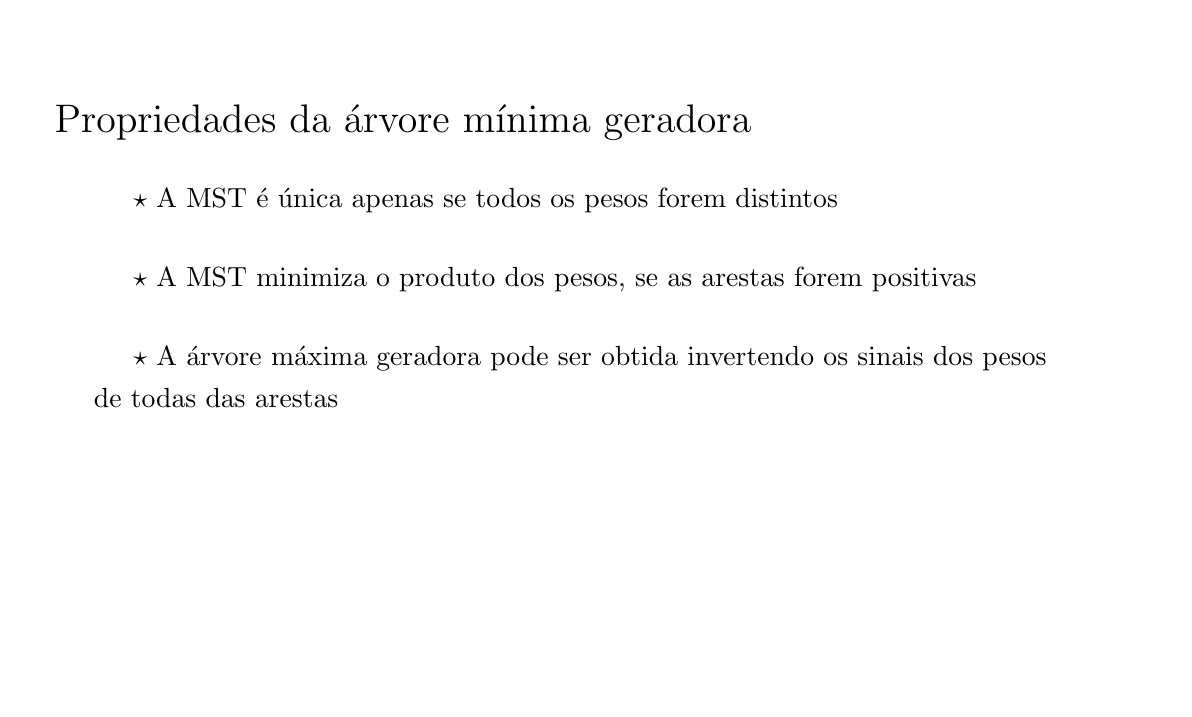
\begin{tikzpicture}
\node[draw,opacity=0] at (0, 0) {x};
\node[draw,opacity=0] at (14, 8) {x};

	\node[anchor=west] (title) at (0.0, 7.0) { \Large \bbbold{Propriedades da árvore mínima geradora} };


	\node[anchor=west] (a) at (1.0, 6.0) { $\star$ \bbtext{A MST é única apenas se todos os pesos forem distintos} };

	\node[anchor=west] (b) at (1.0, 5.0) { $\star$ \bbtext{A MST minimiza o produto dos pesos, se as arestas forem positivas} };


	\node[anchor=west] (c) at (1.0, 4.0) { $\star$ \bbtext{A árvore máxima geradora pode ser obtida invertendo os sinais dos pesos} };

	\node[anchor=west] (c1) at (0.5, 3.5) { \bbtext{de todas das arestas} };


\end{tikzpicture}
\end{frame}
\begin{frame}[plain,t]
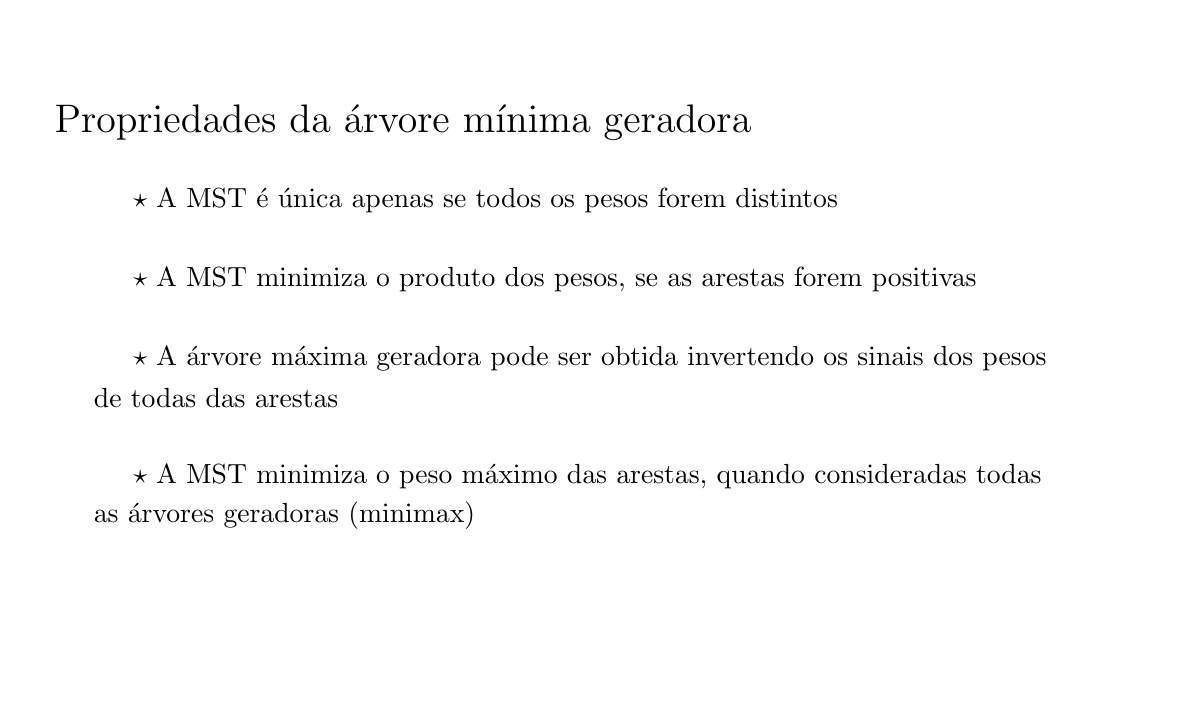
\begin{tikzpicture}
\node[draw,opacity=0] at (0, 0) {x};
\node[draw,opacity=0] at (14, 8) {x};

	\node[anchor=west] (title) at (0.0, 7.0) { \Large \bbbold{Propriedades da árvore mínima geradora} };


	\node[anchor=west] (a) at (1.0, 6.0) { $\star$ \bbtext{A MST é única apenas se todos os pesos forem distintos} };

	\node[anchor=west] (b) at (1.0, 5.0) { $\star$ \bbtext{A MST minimiza o produto dos pesos, se as arestas forem positivas} };


	\node[anchor=west] (c) at (1.0, 4.0) { $\star$ \bbtext{A árvore máxima geradora pode ser obtida invertendo os sinais dos pesos} };

	\node[anchor=west] (c1) at (0.5, 3.5) { \bbtext{de todas das arestas} };



	\node[anchor=west] (d) at (1.0, 2.5) { $\star$ \bbtext{A MST minimiza o peso máximo das arestas, quando consideradas todas} };

	\node[anchor=west] (d1) at (0.5, 2.0) { \bbtext{as árvores geradoras (minimax)} };

\end{tikzpicture}
\end{frame}
\begin{frame}[plain,t]
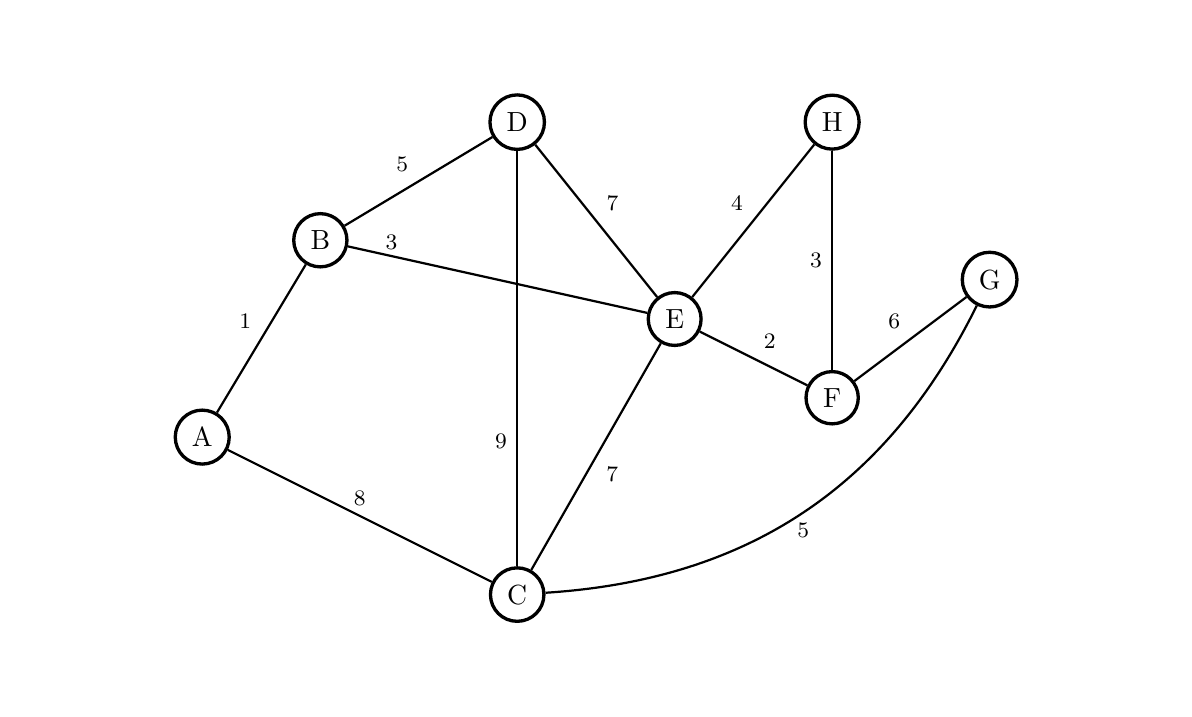
\begin{tikzpicture}
\node[draw,opacity=0] at (0, 0) {x};
\node[draw,opacity=0] at (14, 8) {x};

	\node[draw,very thick,circle] (nodeA) at (2.0, 3.0) { \bbtext{A} };

	\node[draw,very thick,circle] (nodeB) at (3.5, 5.5) { \bbtext{B} };

	\node[draw,very thick,circle] (nodeC) at (6.0, 1.0) { \bbtext{C} };

	\node[draw,very thick,circle] (nodeD) at (6.0, 7.0) { \bbtext{D} };

	\node[draw,very thick,circle] (nodeE) at (8.0, 4.5) { \bbtext{E} };

	\node[draw,very thick,circle] (nodeF) at (10.0, 3.5) { \bbtext{F} };

	\node[draw,very thick,circle] (nodeG) at (12.0, 5.0) { \bbtext{G} };

	\node[draw,very thick,circle] (nodeH) at (10.0, 7.0) { \bbtext{H} };

	\draw[thick](nodeA) to node[above left] { \footnotesize \bbinfo{1} } (nodeB);

	\draw[thick](nodeA) to node[above] { \footnotesize \bbinfo{8} } (nodeC);

	\draw[thick](nodeB) to node[above left] { \footnotesize \bbinfo{5} } (nodeD);

	\draw[thick](nodeB) to node[above left,pos=0.2] { \footnotesize \bbinfo{3} } (nodeE);

	\draw[thick](nodeC) to node[left,pos=0.3] { \footnotesize \bbinfo{9} } (nodeD);

	\draw[thick](nodeC) to node[below right] { \footnotesize \bbinfo{7} } (nodeE);

	\draw[thick](nodeC) to [bend right] node[below] { \footnotesize \bbinfo{5} } (nodeG);

	\draw[thick](nodeD) to node[above right] { \footnotesize \bbinfo{7} } (nodeE);

	\draw[thick](nodeE) to node[above right] { \footnotesize \bbinfo{2} } (nodeF);

	\draw[thick](nodeE) to node[above left] { \footnotesize \bbinfo{4} } (nodeH);

	\draw[thick](nodeF) to node[above left] { \footnotesize \bbinfo{6} } (nodeG);

	\draw[thick](nodeF) to node[left] { \footnotesize \bbinfo{3} } (nodeH);

\end{tikzpicture}
\end{frame}
\begin{frame}[plain,t]
\begin{tikzpicture}
\node[draw,opacity=0] at (0, 0) {x};
\node[draw,opacity=0] at (14, 8) {x};

	\node[draw,very thick,circle] (nodeA) at (2.0, 3.0) { \bbtext{A} };

	\node[draw,very thick,circle] (nodeB) at (3.5, 5.5) { \bbtext{B} };

	\node[draw,very thick,circle] (nodeC) at (6.0, 1.0) { \bbtext{C} };

	\node[draw,very thick,circle] (nodeD) at (6.0, 7.0) { \bbtext{D} };

	\node[draw,very thick,circle] (nodeE) at (8.0, 4.5) { \bbtext{E} };

	\node[draw,very thick,circle] (nodeF) at (10.0, 3.5) { \bbtext{F} };

	\node[draw,very thick,circle] (nodeG) at (12.0, 5.0) { \bbtext{G} };

	\node[draw,very thick,circle] (nodeH) at (10.0, 7.0) { \bbtext{H} };

	\draw[thick](nodeA) to node[above left] { \footnotesize \bbinfo{1} } (nodeB);

	\draw[thick,very thick,dashed,color=BBCyan](nodeA) to node[above] { \footnotesize \bbinfo{8} } (nodeC);

	\draw[thick,very thick,dashed,color=BBCyan](nodeB) to node[above left] { \footnotesize \bbinfo{5} } (nodeD);

	\draw[thick](nodeB) to node[above left,pos=0.2] { \footnotesize \bbinfo{3} } (nodeE);

	\draw[thick,very thick,dashed,color=BBCyan](nodeC) to node[left,pos=0.3] { \footnotesize \bbinfo{9} } (nodeD);

	\draw[thick](nodeC) to node[below right] { \footnotesize \bbinfo{7} } (nodeE);

	\draw[thick,very thick,dashed,color=BBCyan](nodeC) to [bend right] node[below] { \footnotesize \bbinfo{5} } (nodeG);

	\draw[thick,very thick,dashed,color=BBCyan](nodeD) to node[above right] { \footnotesize \bbinfo{7} } (nodeE);

	\draw[thick](nodeE) to node[above right] { \footnotesize \bbinfo{2} } (nodeF);

	\draw[thick,very thick,dashed,color=BBCyan](nodeE) to node[above left] { \footnotesize \bbinfo{4} } (nodeH);

	\draw[thick,very thick,dashed,color=BBCyan](nodeF) to node[above left] { \footnotesize \bbinfo{6} } (nodeG);

	\draw[thick](nodeF) to node[left] { \footnotesize \bbinfo{3} } (nodeH);









	\node[anchor=west] (info) at (0.0, 7.0) { \footnotesize \bbtext{Árvore geradora máxima} };

\end{tikzpicture}
\end{frame}
\begin{frame}[plain,t]
\begin{tikzpicture}
\node[draw,opacity=0] at (0, 0) {x};
\node[draw,opacity=0] at (14, 8) {x};

	\node[anchor=west] (title) at (0.0, 6.0) { \Large \bbbold{Subgrafo gerador mínimo} };

\end{tikzpicture}
\end{frame}
\begin{frame}[plain,t]
\begin{tikzpicture}
\node[draw,opacity=0] at (0, 0) {x};
\node[draw,opacity=0] at (14, 8) {x};

	\node[anchor=west] (title) at (0.0, 6.0) { \Large \bbbold{Subgrafo gerador mínimo} };


	\node[anchor=west] (a) at (1.0, 5.0) { \bbtext{Seja $G(V, E)$ um grafo ponderado e $X\subset E$. O \bbbold{subgrafo gerador mínimo}} };

	\node[anchor=west] (b) at (0.5, 4.25) { \bbtext{$S_X(V, E')$ de $G$ é o subgrafo de $S_X$ de $G$, de custo mínimo, tal que $X \subseteq E'$.} };

\end{tikzpicture}
\end{frame}
\begin{frame}[plain,t]
\begin{tikzpicture}
\node[draw,opacity=0] at (0, 0) {x};
\node[draw,opacity=0] at (14, 8) {x};

	\node[draw,very thick,circle] (nodeA) at (2.0, 3.0) { \bbtext{A} };

	\node[draw,very thick,circle] (nodeB) at (3.5, 5.5) { \bbtext{B} };

	\node[draw,very thick,circle] (nodeC) at (6.0, 1.0) { \bbtext{C} };

	\node[draw,very thick,circle] (nodeD) at (6.0, 7.0) { \bbtext{D} };

	\node[draw,very thick,circle] (nodeE) at (8.0, 4.5) { \bbtext{E} };

	\node[draw,very thick,circle] (nodeF) at (10.0, 3.5) { \bbtext{F} };

	\node[draw,very thick,circle] (nodeG) at (12.0, 5.0) { \bbtext{G} };

	\node[draw,very thick,circle] (nodeH) at (10.0, 7.0) { \bbtext{H} };

	\draw[thick](nodeA) to node[above left] { \footnotesize \bbinfo{1} } (nodeB);

	\draw[thick](nodeA) to node[above] { \footnotesize \bbinfo{8} } (nodeC);

	\draw[thick](nodeB) to node[above left] { \footnotesize \bbinfo{5} } (nodeD);

	\draw[thick](nodeB) to node[above left,pos=0.2] { \footnotesize \bbinfo{3} } (nodeE);

	\draw[thick,very thick,dashed,color=BBRed](nodeC) to node[left,pos=0.3] { \footnotesize \bbinfo{9} } (nodeD);

	\draw[thick,very thick,dashed,color=BBRed](nodeC) to node[below right] { \footnotesize \bbinfo{7} } (nodeE);

	\draw[thick](nodeC) to [bend right] node[below] { \footnotesize \bbinfo{5} } (nodeG);

	\draw[thick,very thick,color=BBRed,dashed](nodeD) to node[above right] { \footnotesize \bbinfo{7} } (nodeE);

	\draw[thick](nodeE) to node[above right] { \footnotesize \bbinfo{2} } (nodeF);

	\draw[thick](nodeE) to node[above left] { \footnotesize \bbinfo{4} } (nodeH);

	\draw[thick](nodeF) to node[above left] { \footnotesize \bbinfo{6} } (nodeG);

	\draw[thick](nodeF) to node[left] { \footnotesize \bbinfo{3} } (nodeH);


\end{tikzpicture}
\end{frame}
\begin{frame}[plain,t]
\begin{tikzpicture}
\node[draw,opacity=0] at (0, 0) {x};
\node[draw,opacity=0] at (14, 8) {x};

	\node[draw,very thick,circle] (nodeA) at (2.0, 3.0) { \bbtext{A} };

	\node[draw,very thick,circle] (nodeB) at (3.5, 5.5) { \bbtext{B} };

	\node[draw,very thick,circle] (nodeC) at (6.0, 1.0) { \bbtext{C} };

	\node[draw,very thick,circle] (nodeD) at (6.0, 7.0) { \bbtext{D} };

	\node[draw,very thick,circle] (nodeE) at (8.0, 4.5) { \bbtext{E} };

	\node[draw,very thick,circle] (nodeF) at (10.0, 3.5) { \bbtext{F} };

	\node[draw,very thick,circle] (nodeG) at (12.0, 5.0) { \bbtext{G} };

	\node[draw,very thick,circle] (nodeH) at (10.0, 7.0) { \bbtext{H} };

	\draw[thick,very thick,dashed,color=BBCyan](nodeA) to node[above left] { \footnotesize \bbinfo{1} } (nodeB);

	\draw[thick](nodeA) to node[above] { \footnotesize \bbinfo{8} } (nodeC);

	\draw[thick](nodeB) to node[above left] { \footnotesize \bbinfo{5} } (nodeD);

	\draw[thick,very thick,dashed,color=BBCyan](nodeB) to node[above left,pos=0.2] { \footnotesize \bbinfo{3} } (nodeE);

	\draw[thick,very thick,dashed,color=BBRed](nodeC) to node[left,pos=0.3] { \footnotesize \bbinfo{9} } (nodeD);

	\draw[thick,very thick,dashed,color=BBRed](nodeC) to node[below right] { \footnotesize \bbinfo{7} } (nodeE);

	\draw[thick,very thick,dashed,color=BBCyan](nodeC) to [bend right] node[below] { \footnotesize \bbinfo{5} } (nodeG);

	\draw[thick,very thick,color=BBRed,dashed](nodeD) to node[above right] { \footnotesize \bbinfo{7} } (nodeE);

	\draw[thick,very thick,dashed,color=BBCyan](nodeE) to node[above right] { \footnotesize \bbinfo{2} } (nodeF);

	\draw[thick](nodeE) to node[above left] { \footnotesize \bbinfo{4} } (nodeH);

	\draw[thick](nodeF) to node[above left] { \footnotesize \bbinfo{6} } (nodeG);

	\draw[thick,very thick,dashed,color=BBCyan](nodeF) to node[left] { \footnotesize \bbinfo{3} } (nodeH);








	\node[anchor=west] (info) at (0.0, 7.0) { \footnotesize \bbtext{Subgrafo gerador mínimo} };

\end{tikzpicture}
\end{frame}
\begin{frame}[plain,t]
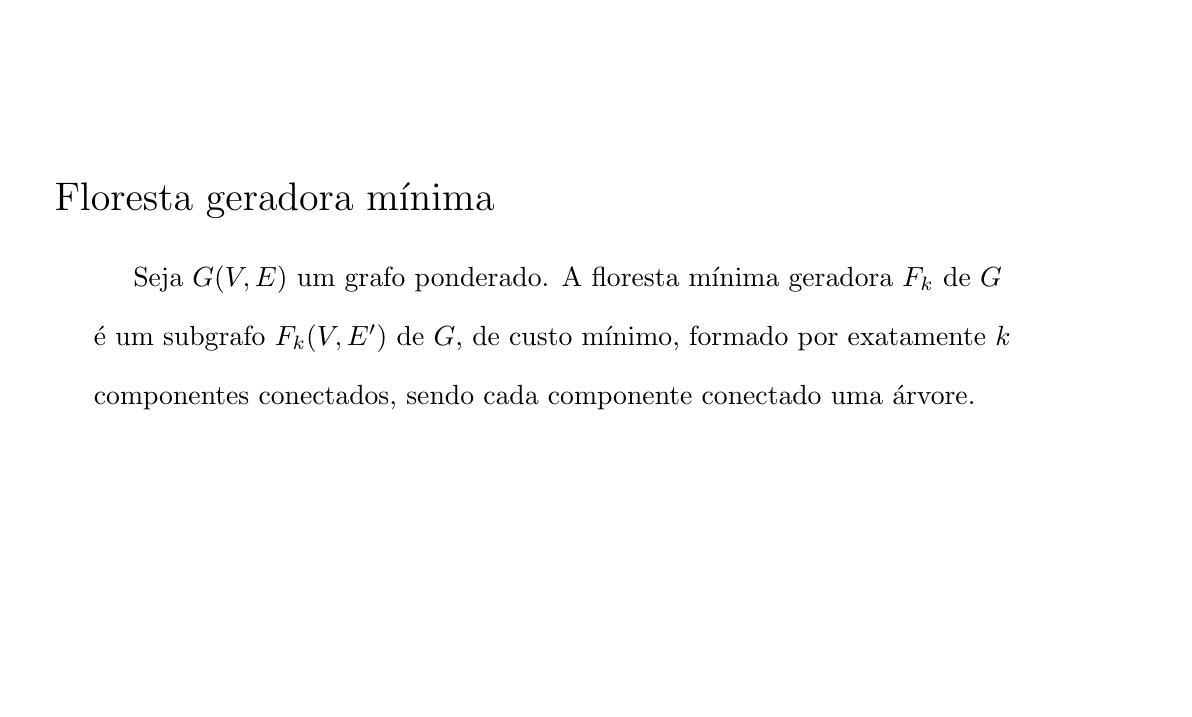
\begin{tikzpicture}
\node[draw,opacity=0] at (0, 0) {x};
\node[draw,opacity=0] at (14, 8) {x};

	\node[anchor=west] (title) at (0.0, 6.0) { \Large \bbbold{Floresta geradora mínima} };

	\node[anchor=west] (a) at (1.0, 5.0) { \bbtext{Seja $G(V, E)$ um grafo ponderado. A \bbbold{floresta mínima geradora} $F_k$ de $G$} };

	\node[anchor=west] (b) at (0.5, 4.25) { \bbtext{é um subgrafo $F_k(V, E')$ de $G$, de custo mínimo, formado por exatamente $k$} };

	\node[anchor=west] (c) at (0.5, 3.5) { \bbtext{componentes conectados, sendo cada componente conectado uma árvore.} };

\end{tikzpicture}
\end{frame}
\begin{frame}[plain,t]
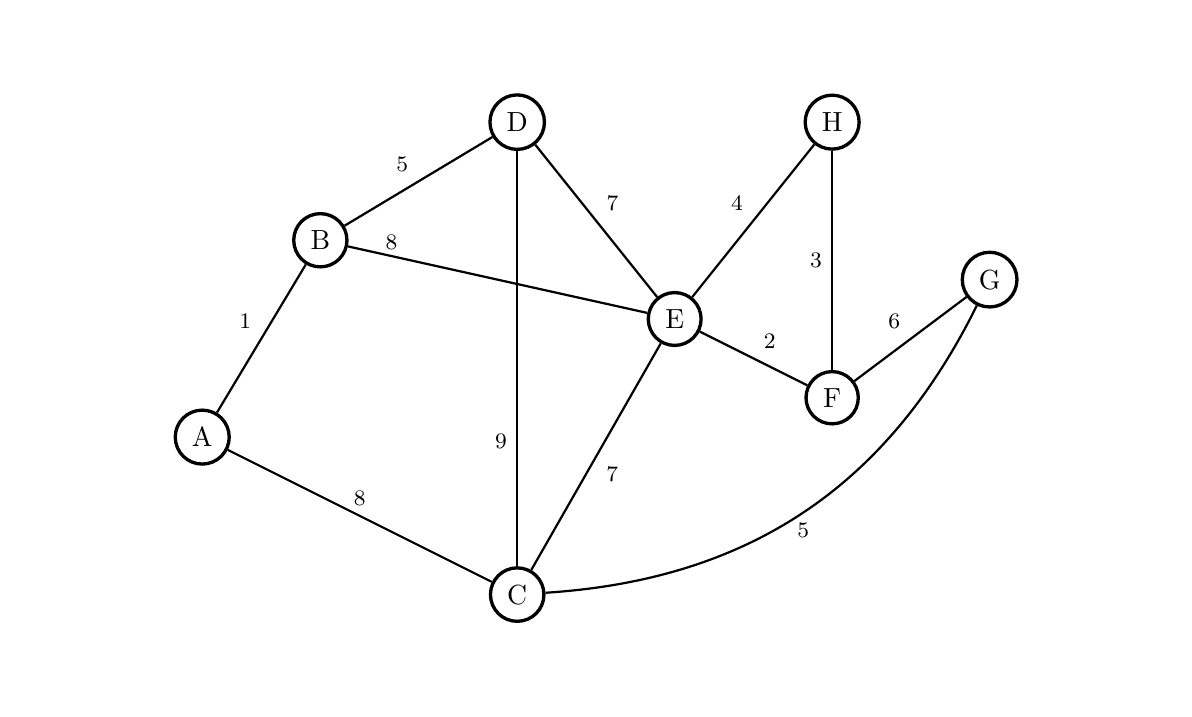
\begin{tikzpicture}
\node[draw,opacity=0] at (0, 0) {x};
\node[draw,opacity=0] at (14, 8) {x};

	\node[draw,very thick,circle] (nodeA) at (2.0, 3.0) { \bbtext{A} };

	\node[draw,very thick,circle] (nodeB) at (3.5, 5.5) { \bbtext{B} };

	\node[draw,very thick,circle] (nodeC) at (6.0, 1.0) { \bbtext{C} };

	\node[draw,very thick,circle] (nodeD) at (6.0, 7.0) { \bbtext{D} };

	\node[draw,very thick,circle] (nodeE) at (8.0, 4.5) { \bbtext{E} };

	\node[draw,very thick,circle] (nodeF) at (10.0, 3.5) { \bbtext{F} };

	\node[draw,very thick,circle] (nodeG) at (12.0, 5.0) { \bbtext{G} };

	\node[draw,very thick,circle] (nodeH) at (10.0, 7.0) { \bbtext{H} };

	\draw[thick](nodeA) to node[above left] { \footnotesize \bbinfo{1} } (nodeB);

	\draw[thick](nodeA) to node[above] { \footnotesize \bbinfo{8} } (nodeC);

	\draw[thick](nodeB) to node[above left] { \footnotesize \bbinfo{5} } (nodeD);

	\draw[thick](nodeB) to node[above left,pos=0.2] { \footnotesize \bbinfo{8} } (nodeE);

	\draw[thick](nodeC) to node[left,pos=0.3] { \footnotesize \bbinfo{9} } (nodeD);

	\draw[thick](nodeC) to node[below right] { \footnotesize \bbinfo{7} } (nodeE);

	\draw[thick](nodeC) to [bend right] node[below] { \footnotesize \bbinfo{5} } (nodeG);

	\draw[thick](nodeD) to node[above right] { \footnotesize \bbinfo{7} } (nodeE);

	\draw[thick](nodeE) to node[above right] { \footnotesize \bbinfo{2} } (nodeF);

	\draw[thick](nodeE) to node[above left] { \footnotesize \bbinfo{4} } (nodeH);

	\draw[thick](nodeF) to node[above left] { \footnotesize \bbinfo{6} } (nodeG);

	\draw[thick](nodeF) to node[left] { \footnotesize \bbinfo{3} } (nodeH);

\end{tikzpicture}
\end{frame}
\begin{frame}[plain,t]
\begin{tikzpicture}
\node[draw,opacity=0] at (0, 0) {x};
\node[draw,opacity=0] at (14, 8) {x};

	\node[draw,very thick,circle] (nodeA) at (2.0, 3.0) { \bbtext{A} };

	\node[draw,very thick,circle] (nodeB) at (3.5, 5.5) { \bbtext{B} };

	\node[draw,very thick,circle] (nodeC) at (6.0, 1.0) { \bbtext{C} };

	\node[draw,very thick,circle] (nodeD) at (6.0, 7.0) { \bbtext{D} };

	\node[draw,very thick,circle] (nodeE) at (8.0, 4.5) { \bbtext{E} };

	\node[draw,very thick,circle] (nodeF) at (10.0, 3.5) { \bbtext{F} };

	\node[draw,very thick,circle] (nodeG) at (12.0, 5.0) { \bbtext{G} };

	\node[draw,very thick,circle] (nodeH) at (10.0, 7.0) { \bbtext{H} };

	\draw[thick,very thick,dashed,color=BBCyan](nodeA) to node[above left] { \footnotesize \bbinfo{1} } (nodeB);

	\draw[thick,opacity=0,very thick,dashed,color=BBCyan](nodeA) to node[above] { \footnotesize \bbinfo{8} } (nodeC);

	\draw[thick,opacity=0](nodeB) to node[above left] { \footnotesize \bbinfo{5} } (nodeD);

	\draw[thick,opacity=0](nodeB) to node[above left,pos=0.2] { \footnotesize \bbinfo{8} } (nodeE);

	\draw[thick,opacity=0](nodeC) to node[left,pos=0.3] { \footnotesize \bbinfo{9} } (nodeD);

	\draw[thick,opacity=0](nodeC) to node[below right] { \footnotesize \bbinfo{7} } (nodeE);

	\draw[thick,very thick,dashed,color=BBGreen](nodeC) to [bend right] node[below] { \footnotesize \bbinfo{5} } (nodeG);

	\draw[thick,opacity=0](nodeD) to node[above right] { \footnotesize \bbinfo{7} } (nodeE);

	\draw[thick,very thick,dashed,color=BBViolet](nodeE) to node[above right] { \footnotesize \bbinfo{2} } (nodeF);

	\draw[thick,opacity=0](nodeE) to node[above left] { \footnotesize \bbinfo{4} } (nodeH);

	\draw[thick,opacity=0](nodeF) to node[above left] { \footnotesize \bbinfo{6} } (nodeG);

	\draw[thick,very thick,dashed,color=BBViolet](nodeF) to node[left] { \footnotesize \bbinfo{3} } (nodeH);







	\node[anchor=west] (info) at (0.0, 7.0) { \footnotesize \bbtext{Floresta mínima geradora $F_4$} };

\end{tikzpicture}
\end{frame}
\begin{frame}[plain,t]
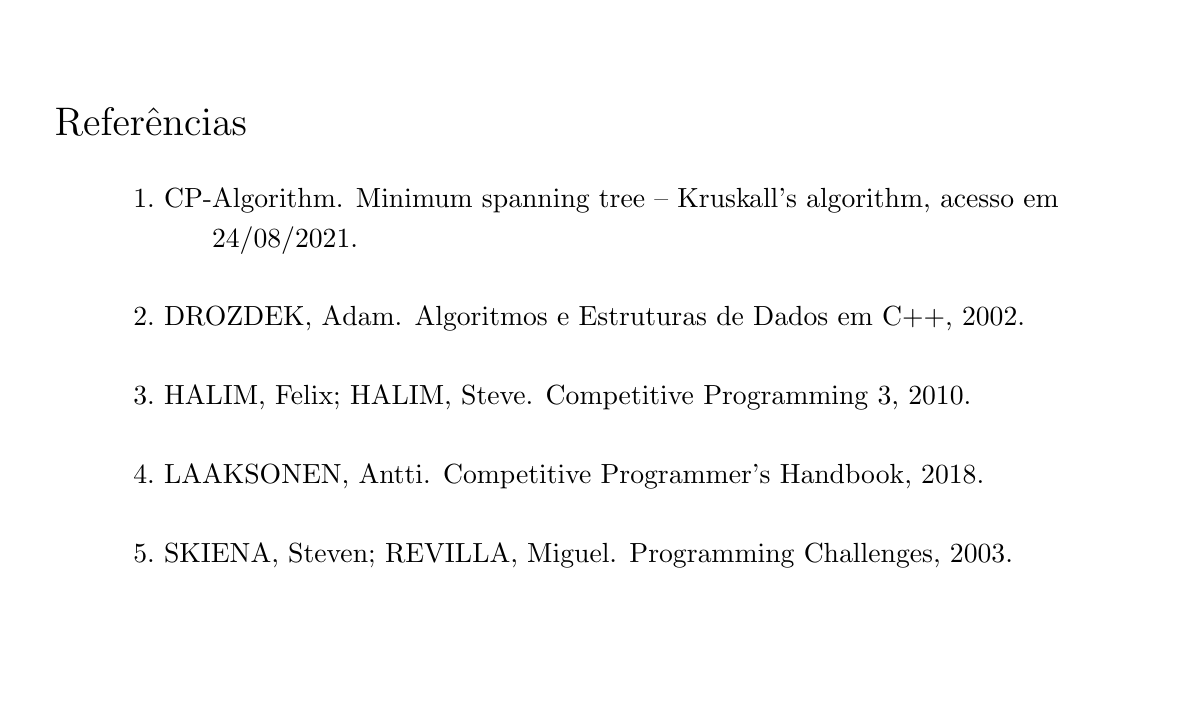
\begin{tikzpicture}
\node[draw,opacity=0] at (0, 0) {x};
\node[draw,opacity=0] at (14, 8) {x};

	\node[anchor=west] (title) at (0.0, 7.0) { \Large \bbbold{Referências} };

	\node[anchor=west] (a) at (1.0, 6.0) { $1.$ \bbtext{\bbbold{CP-Algorithm}. \bbenglish{Minimum spanning tree -- Kruskall's algorithm}, acesso em} };

	\node[anchor=west] (a1) at (2.0, 5.5) { \bbtext{24/08/2021.} };


	\node[anchor=west] (e) at (1.0, 4.5) { $2.$ \bbbold{DROZDEK}, \bbtext{Adam}. \bbenglish{Algoritmos e Estruturas de Dados em C++,} \bbtext{2002.} };


	\node[anchor=west] (b) at (1.0, 3.5) { $3.$ \bbbold{HALIM}, \bbtext{Felix}; \bbbold{HALIM}, \bbtext{Steve}. \bbenglish{Competitive Programming 3,} \bbtext{2010.} };

	\node[anchor=west] (c) at (1.0, 2.5) { $4.$ \bbbold{LAAKSONEN}, \bbtext{Antti}. \bbenglish{Competitive Programmer's Handbook,} \bbtext{2018.} };

	\node[anchor=west] (d) at (1.0, 1.5) { $5.$ \bbbold{SKIENA}, \bbtext{Steven}; \bbbold{REVILLA}, \bbtext{Miguel}. \bbenglish{Programming Challenges,} \bbtext{2003.} };

\end{tikzpicture}
\end{frame}
\end{document}
